\documentclass[t, aspectratio=169, dvipdfmx]{beamer}

\usepackage{url}
\usepackage{hyperref, pxjahyper}
\usepackage{cite}
\usepackage{graphicx}
\usepackage{amsmath, amssymb}
\usepackage{tcolorbox, xcolor}
\usepackage{multicol}

\setbeamertemplate{navigation symbols}{}
\usetheme{AnnArbor}
\usecolortheme{beaver}
\usefonttheme{professionalfonts}

\setbeamertemplate{items}[default]
\setbeamercolor{structure}{fg=darkred}
\setbeamercolor{block title}{fg=white, bg=darkred}
\setbeamercolor{block body}{fg=black, bg=red!10}

\hypersetup{
  colorlinks=true,
}

\title[競プロ体験会]{競技プログラミングを始めよう}
\author{終に鮭}
\institute[OUCRC]{電子計算機研究会}
\date[12/2]{December 2, 2020}

\begin{document}
\frame{\titlepage}

\begin{frame}
  \frametitle{自己紹介}
  \begin{itemize}
    \item 終に鮭
    \item 情報系学科1回生
    \item 競プロ歴8ヶ月(最初のコンテストは4/4のABC161)
    \begin{itemize}
      \item AtCoderしかやってない
      \item 現在のレートは\textcolor{green!50!black}{877}
      \item ごくまれにyukicoderの問題も解く
    \end{itemize}
    \item プログラミング歴は4~5年(?)
    \begin{itemize}
      \item 現在メインで使っている言語はPython, C++, JavaScript
      \item 使ったことのある言語はC, Java, Visual Basic, PHP
    \end{itemize}
  \end{itemize}
\end{frame}

\begin{frame}
  \frametitle{今日の内容}
  \begin{multicols}{2}
    \tableofcontents
  \end{multicols}
\end{frame}

\section{競技プログラミングとは?}
\frame{\sectionpage}

\begin{frame}[c]
  \frametitle{競技プログラミングとは}
  \center{\huge プログラミング早解きコンテストのこと!!}
\end{frame}

\subsection{競プロのいいところ}
\begin{frame}
  \frametitle{競プロのいいところ}
  \begin{itemize}
    \item プログラムが書けるようになる
    \begin{itemize}
      \item 化生の友人(未経験)にAtCoderを教えたらプログラミング1が楽単になった
    \end{itemize}
    \item アルゴリズム・データ構造を学べる
    \begin{itemize}
      \item 次回があればこの部分を掘り下げて勉強会を開くかも
    \end{itemize}
    \item 計算量を意識して書くようになる
    \begin{itemize}
      \item 逆に、$1 \leq N \leq 10^6$なら$O(N \log N)$で2秒に間に合うな、とメタ読みできる
    \end{itemize}
    \item 数学力がつく
    \item 就活に役立つことがある(らしい)
    \begin{itemize}
      \item レートが実力の証明になる
    \end{itemize}
  \end{itemize}
\end{frame}

\subsection{コンテストの形式}
\begin{frame}
  \frametitle{コンテストの形式}
  参加者全員に同じ課題が与えられ、より早く要求を満たすプログラムを記述することを競う
  \begin{itemize}
    \item \textcolor{red}{アルゴ:短時間、最適解が出せる}
    \item マラソン:中長時間、最適解を目指す
    \item コードゴルフ:より短いコードを記述することを競う
  \end{itemize}
\end{frame}

\subsection{オンラインジャッジ}
\begin{frame}
  \frametitle{オンラインジャッジ}
  \begin{itemize}
    \item \textcolor{red}{\href{https://atcoder.jp/home}{AtCoder}(日本):週1,2回、全問日本語に対応}
    \item \href{http://codeforces.com/}{CodeForces}(ロシア):開催頻度がすごい
    \item \href{https://www.tc3.co.jp/topcodersrm/}{TopCoder}(アメリカ):マラソンが充実してる
    \item \href{http://judge.u-aizu.ac.jp/onlinejudge/}{Aizu Online Judge}(日本):\href{https://www.ioi-jp.org/}{JOI}や\href{https://icpc.iisf.or.jp/}{ICPC}の過去問が解ける
  \end{itemize}
\end{frame}

\section{AtCoderをやってみよう}
\frame{\sectionpage}

\subsection{対応言語}
\begin{frame}
  \frametitle{対応言語}
  多すぎて \TeX がクラッシュするので一部のみ抜粋(独断で選びました)
  \begin{block}{主な対応言語(ABC183時点)}
    \begin{multicols}{2}
      \begin{itemize}
        \item C / C++
        \item Java
        \item C\#
        \item Rust
        \item Python / PyPy
        \item Cython
        \item JavaScript (Node.js)
        \item PHP
        \item Ruby
        \item Perl
      \end{itemize}
    \end{multicols}
    延べ57言語が使用可能
    \footnote{\url{https://atcoder.jp/contests/abc182/rules}}
  \end{block}
\end{frame}

\subsection{書き方と注意点}
\begin{frame}[containsverbatim]
  \frametitle{プログラムの書き方と注意点}
  \begin{itemize}
    \item 「入力」は標準入力から受け取れる、「出力」は標準出力に出す
    \begin{itemize}
      \item コマンドライン引数は使わない
      \item 標準入出力を備えていない言語の場合はちょっと特殊(practice contest参照)
      \item 例えばJavaScriptでは \verb|/dev/stdin| からファイル入力、\verb|console.log| で出力
    \end{itemize}
    \item (B問題ぐらいから)制約に注意する
    \begin{itemize}
      \item 算術オーバーフロー
      \begin{itemize}
        \item 黒魔法 \verb|#define int long long|
      \end{itemize}
      \item 実行時間制限超過(TLE:Time Limit Exceeded)
      \begin{itemize}
        \item 1秒間に処理できる量は$10^7$から$10^8$ステップ程度
      \end{itemize}
      \item スタックオーバーフロー
      \begin{itemize}
        \item 再帰の制限は緩められる場合がある
      \end{itemize}
      \item \verb|out_of_range|
    \end{itemize}
  \end{itemize}
\end{frame}

\subsection{提出の練習}
\begin{frame}
  \frametitle{提出の練習}
  \begin{itemize}
    \item 常設中のコンテストから\href{https://atcoder.jp/contests/practice}{practice contest}に飛ぶ
    \item 問題タブから「A - Welcome to AtCoder」を選んで解いてみよう
    \begin{itemize}
      \item 自前のエディタで書くのがおすすめ
      \item 事前調査で回答いただいた言語のサンプルを\href{https://github.com/AAAR-Salmon/procon/tree/main/introduction/sample_practice}{ここ}に用意してあります
    \end{itemize}
  \end{itemize}
  \begin{figure}
    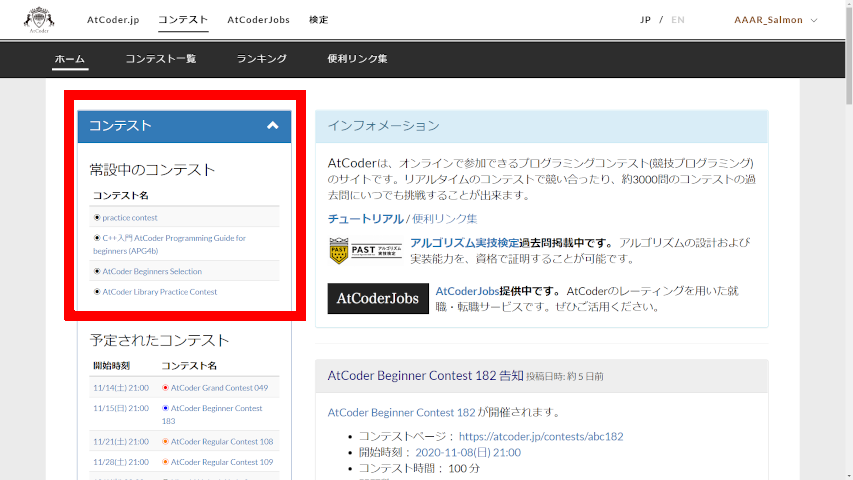
\includegraphics[height=120pt]{atcoder_home.png}
    \caption{AtCoderのコンテストトップページ}
    \label{practice_contest}
  \end{figure}
\end{frame}

\begin{frame}
  \frametitle{提出の練習}
  \begin{itemize}
    \item \textcolor{red}{必ずコードテストする}
    \begin{itemize}
      \item 手元の実行環境を使う
      \item AtCoderのコードテスト機能を使う
    \end{itemize}
    \item 問題ページ下部から提出
  \end{itemize}
\end{frame}

\subsection{典型問題を解いてみよう}
\begin{frame}
  \frametitle{「いかにも競プロ」な問題を解いてみよう}
  \begin{itemize}
    \item どんな問題?
    \begin{itemize}
      \item 文字列操作系問題
      \item 数学の問題
      \begin{itemize}
        \item 小数の計算、幾何、方程式、数え上げ
      \end{itemize}
      \item データ構造を活かす問題
      \begin{itemize}
        \item 配列、集合、スタック・キュー、Union-Find、全域木
      \end{itemize}
      \item 典型アルゴリズムを使う問題
      \begin{itemize}
        \item ソート、探索、累積和、しゃくとり法、いもす法、動的計画法、貪欲法、最短経路問題、最大流問題
      \end{itemize}
    \end{itemize}
  \end{itemize}
\end{frame}

\begin{frame}
  \frametitle{初心者におすすめの問題}
  \begin{itemize}
    \item \href{https://kenkoooo.com/atcoder}{AtCoder Problems}(有志サイト)にバーチャルコンテストを用意したのでやってみよう
    \item 制限時間は1時間
    \item 全問解ききることは想定していないので解けそうな問題から解いてください
    \item インターネットや本で調べてもOK
    \item 全問解説すると時間がかかるので、全員解けた問題と聞いても誰もわからなさそうな問題は解説しません
  \end{itemize}
\end{frame}

\subsection{解説}
\begin{frame}[c]
  \frametitle{解説}
  \center{\huge 解説を始めます}
\end{frame}

\begin{frame}
  \frametitle{配点基準}
  \begin{table}
    \caption{今回採用した配点の基準}
    \label{points}
    \begin{tabular}{ccc}\hline
      配点 & 問題数 & 問題の要素 \\ \hline
      50 & 3 & \begin{tabular}{c}
        if文のみで解ける \\
        数学的考察が不要
      \end{tabular} \\ \hline
      100 & 4 & \begin{tabular}{c}
        if文のみで解けるが、場合分けが難しい \\
        文字列操作が必要 \\
        簡単な数学的要素が含まれる
      \end{tabular} \\ \hline
      200 & 7 & \begin{tabular}{c}
        配列を扱う \\
        ループまたは再帰関数が必要 \\
        単純な多重ループが必要 \\
        小数を扱う \\
        数学的考察が含まれる
      \end{tabular} \\ \hline
    \end{tabular}
  \end{table}
\end{frame}

\begin{frame}
  \frametitle{配点基準}
  \begin{table}
    \caption{今回採用した配点の基準}
    \label{points}
    \begin{tabular}{ccc}\hline
      配点 & 問題数 & 問題の要素 \\ \hline
      300 & 3 & \begin{tabular}{c}
        ナイーブな実装が通用しない \\
        コーナーケースへの対応が必要
      \end{tabular} \\ \hline
      400 & 3 & \begin{tabular}{c}
        特殊なデータ構造を用いる \\
        比較的複雑な典型アルゴリズムを用いる \\
        $\mod 10^9+7$ \\
        複合的なスキルが必要
      \end{tabular} \\ \hline
    \end{tabular}
  \end{table}
\end{frame}

\begin{frame}
  \frametitle{ABC Swap}
  \begin{table}
    \caption{箱とその中身}
    \begin{minipage}{0.2\hsize}
      \begin{center}
        \begin{tabular}{|c|c|c|} \hline
          A & X \\ \hline
          B & Y \\ \hline
          C & Z \\ \hline
        \end{tabular}
      \end{center}
    \end{minipage}
    \begin{minipage}{0.2\hsize}
      \begin{center}
        \begin{tabular}{|c|c|c|} \hline
          A & \textcolor{red}{Y} \\ \hline
          B & \textcolor{red}{X} \\ \hline
          C & Z \\ \hline
        \end{tabular}
      \end{center}
    \end{minipage}
    \begin{minipage}{0.2\hsize}
      \begin{center}
        \begin{tabular}{|c|c|c|} \hline
          A & \textcolor{red}{Z} \\ \hline
          B & X \\ \hline
          C & \textcolor{red}{Y} \\ \hline
        \end{tabular}
      \end{center}
    \end{minipage}
  \end{table}
  \begin{itemize}
    \item swap関数を使ってシミュレーションする
    \item 順番を決め打ちして出力する
  \end{itemize}
\end{frame}

\begin{frame}[containsverbatim]
  \frametitle{AC or WA / Sheep and Wolves}
  \begin{itemize}
    \item $N=M$ / $W \geq S$ か否かを判別するだけ
    \item 条件演算子 \verb|cond ? a : b| を使うと短く書ける
  \end{itemize}
\end{frame}

\section{本番のコンテストについて}
\frame{\sectionpage}

\subsection{参加方法}
\begin{frame}
  \frametitle{参加方法}
  \begin{enumerate}
    \item トップページの左側の「予定されたコンテスト」から選ぶ
    \begin{itemize}
      \item ARC(橙)、AGC(赤)系は難しいのでABC(青)系のコンテストに参加しよう
      \item レートが下がってもいいなら全部参加するのもあり
      \item 現状はNosub撤退すればUnratedになる
      \begin{itemize}
        \item そのためにある程度解けてからまとめて提出する手法がある(tourist出し)
      \end{itemize}
    \end{itemize}
    \item 参加登録する
    \begin{itemize}
      \item 企業コンの場合は個人情報を入力することも
    \end{itemize}
    \item 開催時間にもう一度開く
  \end{enumerate}
\end{frame}

\subsection{おすすめの言語}
\begin{frame}
  \frametitle{おすすめの言語}
  \begin{itemize}
    \item Cが書ける人:C++
    \begin{itemize}
      \item 便利機能が多い
      \begin{itemize}
        \item 文字列型、STLのコンテナクラスや関数、クラス、ラムダ式など
      \end{itemize}
      \item C言語のコードはそのまま動く
      \item 競プロでは一番人口が多い
      \item 最近ACL(AtCoder Library)が導入されてUnion-Findなどを実装しなくて良くなった
    \end{itemize}
    \item ほとんど書けない人:Python
    \begin{itemize}
      \item ライブラリが豊富で便利機能が多い
      \begin{itemize}
        \item range型、ジェネレータ、numpyモジュール
      \end{itemize}
      \item Cと比べると遅いが、現状解けない問題は報告されていない
    \end{itemize}
    \item 速度狂:Rust
    \begin{itemize}
      \item C/C++より更に早い
      \item 暗黙の型変換を一切しないのでめっちゃコンパイルエラーが出る
      \item 全ての型の変数はデフォルトでimmutable(書き換え不可)
    \end{itemize}
  \end{itemize}
\end{frame}

\subsection{注意点}
\begin{frame}
  \frametitle{注意点}
  \begin{itemize}
    \item コンテスト開催中にTwitterなどで余計なことは喋らないようにしよう
    \begin{itemize}
      \item 全員に公開されている情報はOK
      \begin{itemize}
        \item 「A問題ACした」は大丈夫、「A問題WA/TLE/REした」はだめ
        \item 「B問題は余弦定理を使う」、「C問題はbit全探索で間に合う」などもだめ
        \item ソースコードを上げたり生配信したりは当然だめ
      \end{itemize}
      \item 詳細はコンテストページ下部の「ルール」から確認できる
    \end{itemize}
    \item 検索や自作ライブラリの使用は自由
    \begin{itemize}
      \item ただしコンテスト中の情報共有は不可
      \item コードスニペットやテンプレートを用意しておくとよい
    \end{itemize}
  \end{itemize}
\end{frame}

\subsection{役に立つツール}
\begin{frame}
  \frametitle{役に立つツール}
  \begin{itemize}
    \item \href{https://kenkoooo.com/atcoder}{AtCoder Problems}
    \begin{itemize}
      \item コンテスト終了後、問題のdifficultyを推定して色で表示してくれる
      \begin{itemize}
        \item APIが提供されているので、AtCoderのページで色付けするスクリプトなども作られている
      \end{itemize}
      \item 過去問が参照しやすい
      \begin{itemize}
        \item 解いたことのある問題が色付けされる
      \end{itemize}
      \item バーチャルコンテストが開催されている
    \end{itemize}
    \item \href{https://www.npmjs.com/package/atcoder-cli}{atcoder-cli}
    \begin{itemize}
      \item \href{https://nodejs.org/ja/}{Node.js}が必要
      \begin{itemize}
        \item \href{https://github.com/online-judge-tools/oj}{online-judge-tools}が必要で、online-judge-toolsの利用には\href{https://www.python.jp/}{Python3}が必要
      \end{itemize}
      \item ディレクトリの作成、実行テスト、提出がコマンドラインでできるツール
      \item 問題を選択するとサンプルケースを拾ってきてコマンド一つでテストできる
    \end{itemize}
  \end{itemize}
\end{frame}

\end{document}
